\documentclass[12pt]{article}
\usepackage{hyperref}
\usepackage{parskip}
\usepackage{graphicx}
\usepackage{geometry}
\usepackage{setspace}
\usepackage{listings}
%\usepackage{esstixfrak}
%\usepackage{pxtx-frak}
\usepackage{pgothic}
\usepackage{natbib}
\usepackage{amsmath}
\usepackage{amssymb}
\usepackage{url}
\usepackage[english]{babel}
\usepackage[sf]{titlesec}
%\usepackage{cite}
\usepackage{mathptmx}
\usepackage{pdflscape}
\usepackage{array}
\usepackage{tikz}
\usepackage[utf8]{inputenc}
\usepackage{todonotes}
\usepackage{subfigure}
\usetikzlibrary{chains, shapes, backgrounds}

\usetikzlibrary{positioning} 
\usetikzlibrary{shadows}
\usetikzlibrary{shapes}
\usetikzlibrary{shadings}


\newcommand\embeddedsys[3]{
  \begin{scope}[xshift=#1, yshift=#2]
      \draw[rounded corners, drop shadow, shade] (-1.5cm, -1.5cm) rectangle (1.5cm ,1.5cm);
      \node[above] at (0cm, 1.5cm) {\small{Embedded System}};
      \node[rounded corners, rectangle, draw, above, rotate=-90] (#3db) at (-1.4cm, 0cm) {\tiny{Database}};
      \node[rounded corners, rectangle, draw, above] (#3web) at (0cm, -1.4cm) {\tiny{Web Daemon}};
      \node[rounded corners, rectangle, draw, below] (#3sync) at (0cm, 1.4cm) {\tiny{Syncer Daemon}};
      \node[rounded corners, rectangle, draw, above, rotate=90] (#3tor) at (1.4cm, 0cm) {\tiny{TOR Daemon}};
  \end{scope} 
}

\newcommand\rembeddedsys[3]{
  \begin{scope}[xshift=#1, yshift=#2]
      \draw[rounded corners, drop shadow, shade] (-1.5cm, -1.5cm) rectangle (1.5cm ,1.5cm);
      \node[above] at (0cm, 1.5cm) {\small{Embedded System}};
      \node[rounded corners, rectangle, draw, above, rotate=-90] (#3tor) at (-1.4cm, 0cm) {\tiny{TOR Daemon}};
      \node[rounded corners, rectangle, draw, above] (#3web) at (0cm, -1.4cm) {\tiny{Web Daemon}};
      \node[rounded corners, rectangle, draw, below] (#3sync) at (0cm, 1.4cm) {\tiny{Syncer Daemon}};
      \node[rounded corners, rectangle, draw, above, rotate=90] (#3db) at (1.4cm, 0cm) {\tiny{Database}};
  \end{scope} 
}


\usepackage{bera}% optional: just to have a nice mono-spaced font
\usepackage{listings}
\usepackage{xcolor}

\colorlet{punct}{red!60!black}
\definecolor{background}{HTML}{EEEEEE}
\definecolor{delim}{RGB}{20,105,176}
\colorlet{numb}{magenta!60!black}

\lstdefinelanguage{json}{
    basicstyle=\normalfont\ttfamily,
    numbers=left,
    numberstyle=\scriptsize,
    stepnumber=1,
    numbersep=8pt,
    showstringspaces=false,
    breaklines=true,
    frame=lines,
    backgroundcolor=\color{background},
    literate=
     *{0}{{{\color{numb}0}}}{1}
      {1}{{{\color{numb}1}}}{1}
      {2}{{{\color{numb}2}}}{1}
      {3}{{{\color{numb}3}}}{1}
      {4}{{{\color{numb}4}}}{1}
      {5}{{{\color{numb}5}}}{1}
      {6}{{{\color{numb}6}}}{1}
      {7}{{{\color{numb}7}}}{1}
      {8}{{{\color{numb}8}}}{1}
      {9}{{{\color{numb}9}}}{1}
      {:}{{{\color{punct}{:}}}}{1}
      {,}{{{\color{punct}{,}}}}{1}
      {\{}{{{\color{delim}{\{}}}}{1}
      {\}}{{{\color{delim}{\}}}}}{1}
      {[}{{{\color{delim}{[}}}}{1}
      {]}{{{\color{delim}{]}}}}{1},
}


\usepackage{graphicx}
\makeatletter
\providecommand{\bigsqcap}{%
  \mathop{%
    \mathpalette\@updown\bigsqcup
  }%
}
\newcommand*{\@updown}[2]{%
  \rotatebox[origin=c]{180}{$\m@th#1#2$}%
}
\makeatother

\geometry{a4paper,margin=1.2in}

\title{\textpgoth{\Huge{Zwiebelnetz}}\\ \small{-Tech Report-}}
\author{Dario Brandes, Thies Johannsen,\\Paul Kröger, Sergej Mann,\\Roman Naumann, Sebastian Thobe}
\date{\today}

\newcommand{\low}{\textbf{Low}\space}
\newcommand{\high}{\textbf{High}\space}
\newcommand{\lub}{\sqcup}
\newcommand{\glb}{\sqcap}
\newcommand{\mayflowto}{\subseteq}
\newcommand{\labelof}[1]{\underline{#1}}
\newcommand{\Zwiebelnetz}{\textpgoth{Zwiebelnetz}~}

\begin{document}

\maketitle

\onehalfspacing

\tableofcontents

\listoftodos
\section{Introduction}

The rise of online communications and social networks affect the way we interact today. A great deal of personal information is stored on electronic devices and transmitted over the Internet.
While the recent revelations by Edward Snowden showed the extent of government agencies spying on personal data, it was understood before by the security community that there is a need to better protect privacy in online communications.

A number of promising projects, such as Tox ~\cite{ToxProject}, were started to thwart prying on user data. We found, however, no project for social networking with a satisfactory focus on privacy.

The Zwiebelnetz, described in this tech report, is a prototype of a social network which seeks to protect user data.

\section{Overview}

The Zwiebelnetz currently provides basic features for social networking, such as contact requests, circle management, posts, comments and profile information.

The data published in the network is hosted in a distributed fashion; each user has an embedded system connected to the internet which stores and serves the data she published.

~\autoref{arch_overview} shows the main components of the Zwiebelnetz:
\begin{description}
\item[Syncer Daemon] Keeps databases of several systems in sync, see \autoref{syncer_protocol}
\item[Tor Damon] Serves as a proxy to the Internet, see \autoref{tor}.
\item[Web Daemon] Serves the web frontend to the local network 	(see ~\autoref{frontend}).
\item[Database] An SQLite3 ~\cite{sqlite} database storing all user content, see \autoref{database}
\end{description}

\begin{landscape}
\begin{figure}[h]
  \centering
    \includegraphics[scale=0.5]{../slides/figures/overview_01.jpg} 
  \caption{Architecture Overview} \label{arch_overview}
\end{figure}
\end{landscape}
  
\section{Network Protocol}
\label{syncer_protocol}
\subsection{Terms}

The following terms will be used in this section:

\begin{description}
\item[syncer daemon] The system process which provides the synchronization hidden service and regularly pulls updates from other syncers.
\item[web daemon] The system process which serves the web interface to the local network.
\item[client] Despite the peer-to-peer nature of the protocol, it is useful to distinguish between the connecting entity (giver) and the serving entity (taker). we describe the \textit{connecting} syncer daemon as the client.
\item[server] The server describes the syncer daemon which handles a connection of a client.
\end{description}

\subsection{Tor Usage}
\label{tor}
The \texttt{syncer daemon} runs on the embedded system, it listens on port $3141$ on localhost only.
Other systems do not communicate directly with the syncer over the Internet, but connect to it via Tor hidden services \cite{TorHiddenServices}. Syncer access the Tor daemon uses the \texttt{SOCKS4a} protocol ~\cite{socks4a}, an extension to the \texttt{SOCKS4} protocol ~\cite{socks4} adding support for hostnames \footnote{The hostname support is required since Tor resolves onion addresses, not IP addresses}.

We use Tor for three reasons:

\begin{enumerate}
\item Network Address Traversal (NAT) and Name Resolution
\item Cryptographic Guarantees
\item Hidden Social Graph
\end{enumerate}

\subsubsection*{NAT and Name Resolution}

The Tor network serves a distributed hash table (DHT) of hidden services' onion addresses. Given an onion address, a client can use the Tor daemon to establish a connection to the hidden service. No DNS name or static IP address is required, all information needed can be found in the Tor DHT. It is common for home users' Internet connectivity to have dynamic IP addresses without a hostname bound to those addresses.

Modern routers as found in home environments commonly use NAT to map the addresses and ports used on the local network to the IP addresses and ports used on the internet. The Tor daemon which provides the hidden service establishes several introductory points through the Tor network and keeps TCP connections to the first node of each path open. This effectively bypasses the NAT barrier so that users of the system do not need to configure their routers to forward specific ports.

\subsection*{Cryptographic Properties}

The tor hidden service protocol provides secrecy, data integrity and authentication ~\cite{Dingledine:2004:TSO:1251375.1251396}. Due to the nature of tor - being an anonymous communication service - the server syncer does not know which system the connection originated from. We therefore implemented a one-directional challenge response protocol, described in section \ref{authentication}, to authenticate the connecting client.

\subsection*{Hidden Social Graph}

The Zwiebelnetz builds an overlay network with a friend-to-friend topology. The social graph of users can easily reconstructed from such connection \mbox{(meta-)data}. Tor's onion routing protects the connection data by attackers being able to observe and manipulate parts of the Internet. The use of Tor as a means to build the friend-to-friend overlay hides the social network from those attackers.

\subsection{Syncer States}

The syncer accepts new connections and waits for further instructions. The ~\autoref{syncer_states} shows the state machine followed by each syncer thread handling a new connection. Terminal states close the connection after the commands of the state were executed.

\begin{figure}[h]
  \centering
    \includegraphics[scale=0.7]{img/syncer.pdf}
  \caption{Architecture Overview} \label{syncer_states}
\end{figure}

Each state is entered upon receiving one more more network messages, see \ref{messages} for a detailed description of each message.
\autoref{network_use_cases} shows how the different components work together in typical use cases like posting comments.

\subsection{Authentication}

\label{authentication}

Some commands require (or behave different after) successful authentication of the client.
Authentication is done via a encryption based public key challenge response protocol \cite{Menezes:1996:HAC:548089:chap10}.

The client requests authentication by sending an \texttt{Auth} package to the server containing the client's \texttt{DER}-encoded public key.

The server calculates the onion address of the public key from the \texttt{Auth} package and checks if a verified \footnote{A verified contact has a status of \texttt{following}, \texttt{pending} or \texttt{success}, but \textit{not} \texttt{open} or \texttt{blocked}} contact with this onion address exists in the database. If no verified contact is found, the connection is closed.

If a verified contact is found, the server generates a $256$ bit long random number $r$ and sends a \texttt{Challenge} message to the client. The challenge consists of the following three parts:

\begin{enumerate}
\item[$H(r)$] The \texttt{SHA-256} hash of $r$
\item[$PK_s$] The \texttt{DER}-encoded PublicKey of the server
\item[$Enc_{PK_c}$] A message which is encrypted using \texttt{RSA-OAEP} mode with \texttt{SHA-224} as the hash function.
\end{enumerate}

The encrypted message contains the following two fields:

\begin{enumerate}
\item[$r$] The 256 bit long random number $r$
\item[$H(PK_s)$] The \texttt{SHA-256} hash of the public key of the server \footnote{The Handbook of Applied Cryptography sends the full public key in the ciphertext instead of it's hash. We only send to hash because of size limitations of \texttt{RSA-OAEP}; we only need to encrypt one block.}
\end{enumerate}

The client decrypts the ciphertext and makes a number of checks before sending a response:

\begin{enumerate}
\item the onion address of $PK_s$ is the same to which the client connected in the first place.
\item Hashing $PK_s$ from the plaintext gives the same hash as the $H(PK_s)$ from the decrypted ciphertext.
\item Hashing $r$ from the ciphertext gives the same $H(r)$ as from the plaintext.
\end{enumerate}

If any of those checks fails the client considers the authentication to have failed and will not produce a response.

Note that $H(R)$ is used as a witness so that the client can verify that the server knows the answer to the challenge. Otherwise it could be possible for the server to abuse the client as a decryption oracle.
$H(PK_s)$ in the encrypted message on the other hand serves as a protection so that the server cannot forward a challenge from another system to the client.

The response only contains $r'$. The server checks that $r = r'$ and sends a \texttt{Success} packet to the client. If $r \neq r'$, the authentication failed and the server closes the connection.

\subsection{Tasks of the individual components involved in the main use cases}
\subsubsection{User published a posts}
\begin{figure}[ht]
  \subfigure[Server side post publication]{
  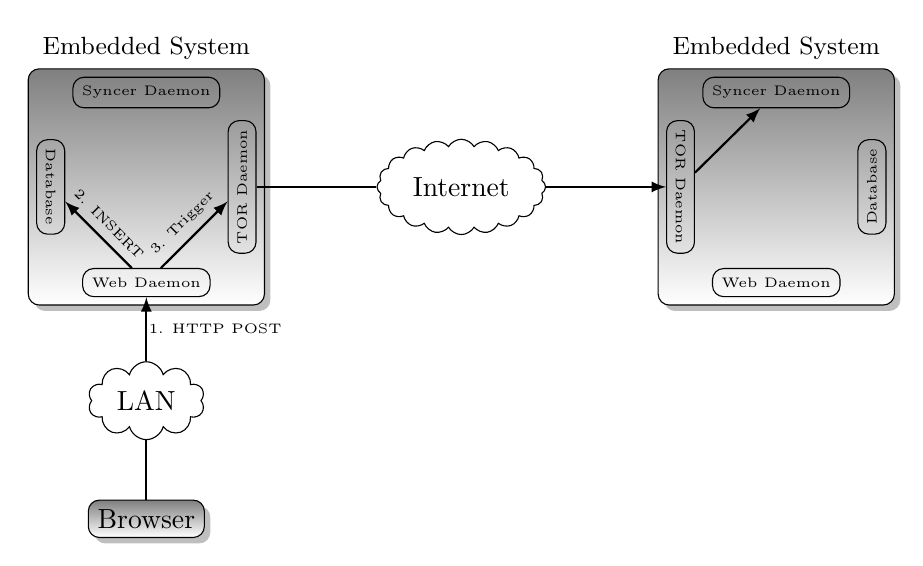
\begin{tikzpicture}
    \embeddedsys{0cm}{0cm}{u1}
    \node[cloud, cloud puffs=20, minimum width=2cm, cloud puff arc=120, draw, aspect=2] (inet) at (4.0cm, 0cm) {Internet};
    \rembeddedsys{8cm}{0cm}{u2}
    
    \node[below of=u1web, node distance=1.5cm, cloud, draw, aspect=2] (u1lan) {LAN};

    \node[below of=u1lan, rounded corners, draw, drop shadow, shade, node distance = 1.5cm] (browser1) {Browser};

    \draw[thick] (browser1.north) -- (u1lan.south);
    \draw[-latex, thick] (u1lan) -- (u1web) node[midway,  right, xshift=-.1cm] {\tiny{1. HTTP POST}};

    \draw[-latex, thick] (u1web) -- (u1db) node[midway, sloped, above] {\tiny{2. INSERT}};

    \draw[-latex, thick] (u1web) -- (u1tor) node[midway, above, sloped] {\tiny{3. Trigger}};
    \draw[thick] (u1tor) -- (inet);
    \draw[thick, -latex] (inet) -- (u2tor);
    \draw[thick, -latex] (u2tor) -- (u2sync);
  \end{tikzpicture}}
  \subfigure[Client side post transmission]{
  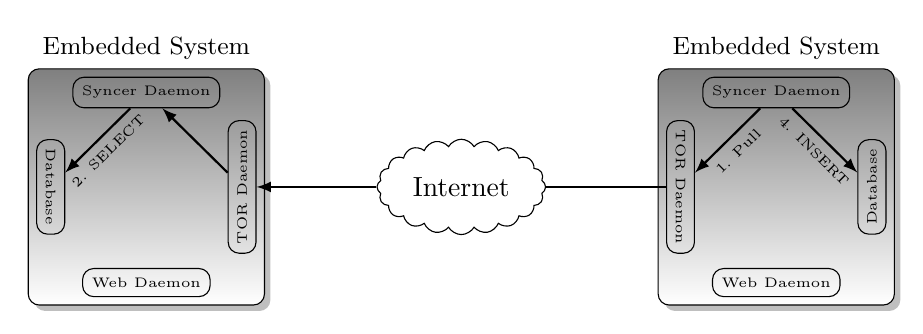
\begin{tikzpicture}
    \embeddedsys{0cm}{0cm}{u1}
    \node[cloud, cloud puffs=20, minimum width=2cm, cloud puff arc=120, draw, aspect=2] (inet) at (4.0cm, 0cm) {Internet};
    \rembeddedsys{8cm}{0cm}{u2}

    \draw[thick, -latex] (u2sync) -- (u2tor) node[sloped, below, midway] {\tiny{1. Pull}};
    \draw[thick] (u2tor) -- (inet);
    \draw[thick, -latex] (inet) -- (u1tor);
    \draw[thick, -latex] (u1tor) -- (u1sync);

    \draw[thick, -latex] (u1sync) -- (u1db) node[sloped,midway, below] {\tiny{2. SELECT}};
    
    \draw[thick, -latex] (u2sync) -- (u2db) node[below, midway, sloped] {\tiny{4. INSERT}};
  \end{tikzpicture}}
  \caption{Post publication}
\end{figure}
When the user posts a message the web browser sends a HTTP POST request to the REST-API.
The REST-API server inserts the post into the database and sends trigger messages to all contacts that are part of the circles the post is publihed in (see figure 3 (a)).
A client who is triggered scans the database for the latest timestemp (\texttt{remote\_published\_at} for posts and \texttt{changed\_at} for profiles) of a post or profile from the contact that send the
trigger message.
Afterwards the client sends a pull request with the determined timestemp to the syncer daemon who send the trigger message.
The syncer daemon who received the pull request scans its database for posts with a \texttt{published\_at} timestamp greater then the timestemp received with the pull request and sends all posts
meeting that condition to the client. The client saves all received posts in its database. For eachs post, the received \texttt{published\_at} timestamp is locally saved as the \texttt{remote\_published\_at}
timestamp (see figure 3 (b)).
\subsubsection{User comments on a post}
\begin{figure}[ht]
  \subfigure[Node a publishes a post to nodes b, c and d]{
    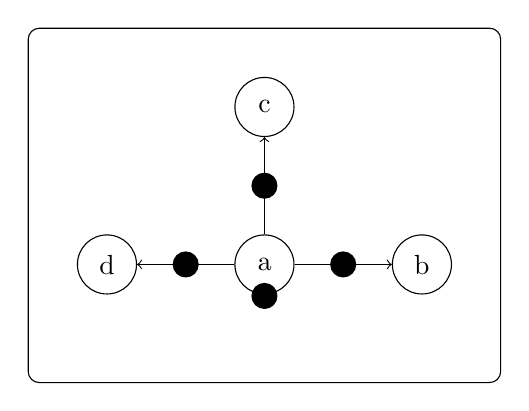
\begin{tikzpicture}
     \draw[rounded corners] (-3cm, -1.5cm) rectangle (3cm, 3cm);
     \node[draw, minimum width=.75cm, circle] (a) at ( 0cm,  0cm)  {a};
     \node[draw, minimum width=.75cm, circle] (b) at ( 2cm,  0cm)  {b};
     \node[draw, minimum width=.75cm, circle] (c) at ( 0cm,  2cm)  {c};
     \node[draw, minimum width=.75cm, circle] (d) at (-2cm,  0cm)  {d};
     \node[circle, fill, below of = a, node distance=.4cm] {};
     
     \draw[->] (a) -- (b) node[midway, circle, fill] {};
     \draw[->] (a) -- (c) node[midway, circle, fill] {};
     \draw[->] (a) -- (d) node[midway, circle, fill] {};
   \end{tikzpicture}
  }\hfill\subfigure[Node b published a comment on the post. The comment is pulled by node a. Node b marks the comment as pending since it has not
  been republished by node a]{
    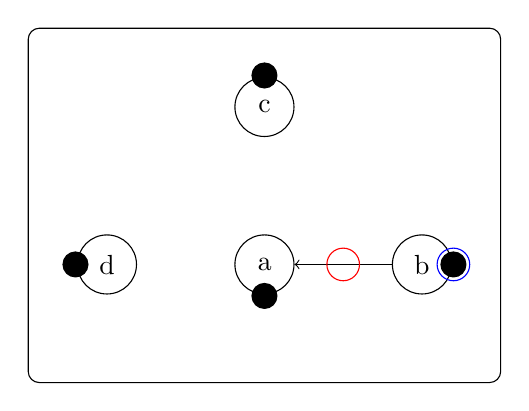
\begin{tikzpicture}
       \draw[rounded corners] (-3cm, -1.5cm) rectangle (3cm, 3cm);
       \node[draw, minimum width=.75cm, circle] (a) at ( 0cm,  0cm)  {a};
       \node[draw, minimum width=.75cm, circle] (b) at ( 2cm,  0cm)  {b};
       \node[draw, minimum width=.75cm, circle] (c) at ( 0cm,  2cm)  {c};
       \node[draw, minimum width=.75cm, circle] (d) at (-2cm,  0cm)  {d};

       \node[circle, fill, below of = a, node distance=.4cm] {};
       \node[circle, fill, right of = b, node distance=.4cm] {};
       \node[circle, fill, above of = c, node distance=.4cm] {};
       \node[circle, fill, left of = d, node distance=.4cm] {};

       \node[circle, draw=blue,right of = b, node distance=.4cm, scale=1.25] {};
       \draw[->] (b) -- (a) node[midway, circle, draw=red, scale=1.25] {};
    \end{tikzpicture}
  }
  \subfigure[Node a publishes the comment to nodes b, c and d]{
    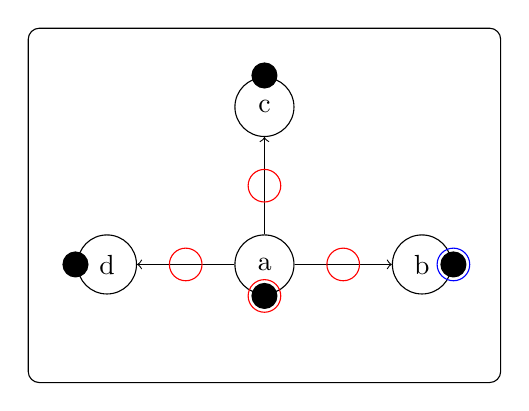
\begin{tikzpicture}
       \draw[rounded corners] (-3cm, -1.5cm) rectangle (3cm, 3cm);
       \node[draw, minimum width=.75cm, circle] (a) at ( 0cm,  0cm)  {a};
       \node[draw, minimum width=.75cm, circle] (b) at ( 2cm,  0cm)  {b};
       \node[draw, minimum width=.75cm, circle] (c) at ( 0cm,  2cm)  {c};
       \node[draw, minimum width=.75cm, circle] (d) at (-2cm,  0cm)  {d};

       \node[circle, fill, below of = a, node distance=.4cm] {};
       \node[circle, fill, right of = b, node distance=.4cm] {};
       \node[circle, fill, above of = c, node distance=.4cm] {};
       \node[circle, fill, left of = d, node distance=.4cm] {};

       \node[circle, draw=blue, right of = b, node distance=.4cm, scale=1.25] {};
       \node[circle, draw=red, below of = a, node distance=.4cm, scale=1.25] {};
       
       \draw[->] (a) -- (b) node[midway, circle, draw=red, scale=1.25] {};
       \draw[->] (a) -- (c) node[midway, circle, draw=red, scale=1.25] {};
       \draw[->] (a) -- (d) node[midway, circle, draw=red, scale=1.25] {};
    \end{tikzpicture}
  }\hfill\subfigure[As node b receives the comment from a, it clears the pending state]{
    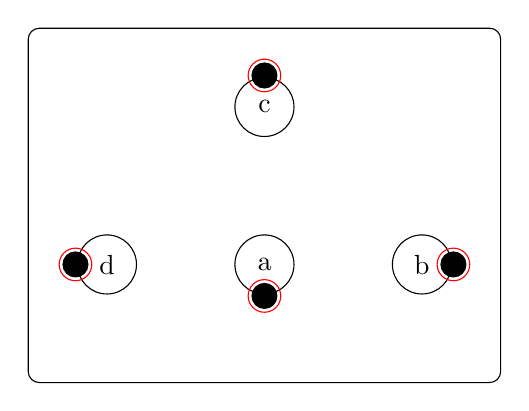
\begin{tikzpicture}
       \draw[rounded corners] (-3cm, -1.5cm) rectangle (3cm, 3cm);
       \node[draw, minimum width=.75cm, circle] (a) at ( 0cm,  0cm)  {a};
       \node[draw, minimum width=.75cm, circle] (b) at ( 2cm,  0cm)  {b};
       \node[draw, minimum width=.75cm, circle] (c) at ( 0cm,  2cm)  {c};
       \node[draw, minimum width=.75cm, circle] (d) at (-2cm,  0cm)  {d};

       \node[circle, fill, below of = a, node distance=.4cm] {};
       \node[circle, fill, right of = b, node distance=.4cm] {};
       \node[circle, fill, above of = c, node distance=.4cm] {};
       \node[circle, fill, left of = d, node distance=.4cm] {};

       \node[circle, draw=red, right of = b, node distance=.4cm, scale=1.25] {};
       \node[circle, draw=red, below of = a, node distance=.4cm, scale=1.25] {};
       \node[circle, draw=red, above of = c, node distance=.4cm, scale=1.25] {};
       \node[circle, draw=red, left of = d, node distance=.4cm, scale=1.25] {};
    \end{tikzpicture}
  }
   \caption{Comment publication}
\end{figure}

If a user comments on a post, the comment is send back to the originator of the post.
The message format and database table for posts and comments is the same. A comment is a post with the \texttt{parent\_id} field set to the id
of the post the comment refers to. On different systems the post ids differ. To refer to the same post on different machines a
SHA-256 hash is used. The hash is computed based on the timestemp, the onion address of the auhor and the content of the post.
After receiving the comment, the post originator distributes the comment to all contacts the post was send to, if the comments TTL field is greater
than zero (see figure 4).


\subsubsection{Contact requests}
If a user adds a new contact, a contact request packet is send to the contacts onion.
The new cotact inserts the requesting contact into its database with its status field set to \texttt{OPEN}.
If the requested user accepts the contact request, the REST-API server sends a trigger packet to the requesting syncer.
Afterwards the triggered syncer tries to authenticate and pull from the triggering syncer. If the authentication is successfull the client syncer
updates the contacts state to \texttt{SUCCESS}.

\subsubsection{Profile information}
Profile information are, like posts, send in reply to a pull request. If the pulling syncer receives the first profile key-value pair it
deletes all profile information in the database from the onion it pulls from, so that fields that are outdated are deleted.
Afterwards the received profiles are inserted into the database.
\subsection{Message Format}

Messages are transmitted over a \texttt{TCP} connection established by the \texttt{TOR} daemon. The messages are encoded using \texttt{JSON} ~\cite{rfc7159} notation. \texttt{JSON} only specifies single messages, we therefore use a simple, binary message format specifying type and length of messages to allow sending multiple \texttt{JSON} messages over a single \texttt{TCP} connection.

\begin{tabular}{|r|l|}
\hline
bytes & field \\\hline\hline
1 & message type \\\hline
4 & message length $n$ in bytes\\\hline
$n$ & json encoded message \\\hline
\end{tabular}

\subsection{Individual Message Formats}

\label{messages}

\subsubsection*{Auth}

\begin{tabular}{l p{.8\textwidth}}
\hline
message type: & $0x41$ ('\textbf{A}') \\
description: & \texttt{Auth} messages are sent by the client to request authentication. They initiate a challenge response authentication \\
encoding: & \texttt{JSON} \textbf{data} \\\hline
\end{tabular}

\texttt{JSON}:

\begin{tabular}{|l|l|}
\hline
type & description \\\hline\hline
binary & \texttt{DER} encoding of the client's public key \\\hline
\end{tabular}

\subsubsection*{Challenge}

\begin{tabular}{l p{.8\textwidth}}
\hline
message type & $0x43$ ('\textbf{C}') \\
description & \texttt{Challenge} messages are sent by the server after receiving an \texttt{Auth} messages of a verified contact. \\
encoding & \texttt{JSON} \textbf{struct} \\
\end{tabular}

The \texttt{JSON} encoding is a \textbf{struct} with the following fields:

\begin{tabular}{|l|l|l|}
\hline
name & type & description \\\hline\hline
HR        & binary & hash of the server's public key \\\hline
PubKey    & binary & \texttt{DER}-encoded server's public key \\\hline
Enc       & binary & ciphertext (see \autoref{authentication}) \\\hline
\end{tabular}


\subsubsection*{Response}

\begin{tabular}{l p{.8\textwidth}}
\hline
message type & $0x52$ ('\textbf{R}') \\
description & \texttt{Response} messages are sent by the client in response to a a \texttt{Challenge} message. \\
encoding & \texttt{JSON} \textbf{data} \\\hline
\end{tabular}

\texttt{JSON}:

\begin{tabular}{|l|l|}
\hline
type & description \\\hline\hline
binary & decrypted 256 bit long random number $r$ \\\hline
\end{tabular}

\subsubsection*{Success}

\begin{tabular}{l p{.8\textwidth}}
\hline
message type & $0x53$ ('\textbf{S}') \\
description & \texttt{Success} messages are sent after successful \texttt{Pull}, \texttt{Trigger}, \texttt{Auth} and \texttt{ContactRequest} messages. \\
encoding & none (no payload) \\\hline
\end{tabular}

\subsubsection*{Trigger}

\begin{tabular}{l p{.8\textwidth}}
\hline
message type & $0x54$ ('\textbf{T}') \\
description & \texttt{Trigger} messages are sent to a server to indicate that a subsequent pull of the server syncer to the client syncer will yield new information. \\
encoding & none (no payload) \\
\end{tabular}

\subsection*{Pull}

\begin{tabular}{l p{.8\textwidth}}
\hline
message type & $0x50$ ('\textbf{P}') \\
description & A syncer can request all posts, comments and profile updates he may see with a \texttt{Pull} message. Without prior authentication, only \texttt{Public} information will be sent to the client. With prior authentication \texttt{Public} information \textit{and} information, which is accesable to any \texttt{circle} of the contact, will be sent. \\
encoding & \texttt{JSON} \textbf{data} \\\hline
\end{tabular}

\texttt{JSON}:

\begin{tabular}{l p{.8\textwidth}}
\hline
type & description \\\hline
number & timestamp (only data newer than this timestamp will be sent by the remote syncer) \\\hline
\end{tabular}

\subsection*{PushPost}

\begin{tabular}{l p{.8\textwidth}}
\hline
message type & $0x51$ ('\textbf{Q}') \\
description & \texttt{PostPost} messages contain a post or comment, they are sent in response to a \texttt{Pull} request. \\
encoding & \texttt{JSON} \textbf{struct} \\\hline
\end{tabular}

The \texttt{JSON} encoding is a \textbf{struct} with the following fields:

\begin{tabular}{|l|l|p{.8\textwidth}|}
\hline
name & type & description \\\hline\hline
Message     & text   & Markdown text of the post or comment. \\\hline
PostedAt    & number & UTC Unix-Timestamp when the post or comment was created. \\\hline
PublishedAt & number & UTC Unix-Timestamp when the \\\hline
TTL         & number & Time-To-Live of the post or comment, may not be forwarded  \\\hline
Author      & text   & The author's onion address of the post or comment \\\hline
Hash        & text   & H(Message, PostedAt, Author's Onion) (\texttt{SHA-256})\\\hline
ParentHash  & text   & The empty string for a post; the hash (see above) of the post to which the comment refers for comments\\\hline
\end{tabular}

\subsection*{PushProfile}

\begin{tabular}{ l p{.8\textwidth} }
\hline
message type & $0x55$ ('\textbf{U}') \\
description & \texttt{PushProfile} messages contain a single profile entry, they are sent in response to a \texttt{Pull} request. \\
encoding & \texttt{JSON} \textbf{struct} \\\hline
\end{tabular}

The \texttt{JSON} encoding is a \textbf{struct} with the following fields:

\begin{tabular}{|l|l|p{.8\textwidth}|}
\hline
name & type & description \\\hline\hline
Key         & text   & The name of the profile entry. \\\hline
Value       & text   & The value of the profile entry. \\\hline
ChangedAt   & number & UTC Unix-Timestamp when the entry was created or changed. \\\hline
\end{tabular}

\subsection*{ContactRequest}

\begin{tabular}{l p{.8\textwidth}}
\hline
message type & $0x42$ ('\textbf{B}') \\
description & \texttt{ContactRequest} messages cause the server to create a new contact for the client with status \texttt{Open}. \\
encoding & \texttt{JSON} \textbf{struct} \\\hline
\end{tabular}

The \texttt{JSON} encoding is a \textbf{struct} with the following fields:

\begin{tabular}{|l|l|p{.8\textwidth}|}
\hline
name & type & description \\\hline\hline
Message   & text & The contact-request message which will be shown to the user of the server. \\\hline
Onion     & text & The onion address of the client. \\\hline
\end{tabular}

\section{Database}
\label{database}
This section describes the most important database tables. Tables that are only needed to represent relations are omitted here.
All database tables described in this section have an id field which is not shown here.   
\subsection{Onion}
An onion represents a tor hidden service onion address.

\begin{tabular}{>{\ttfamily}p{.3\textwidth}>{\ttfamily}p{.1\textwidth}p{.6\textwidth}}
Column Name    & Type & Description \\ \hline \hline
  Onion & text & Tor Onion Address
\end{tabular}

\subsection{Contact}
A contact extends the onion address with personal information.
It has the following columns.

\begin{tabular}{>{\ttfamily}p{.3\textwidth}>{\ttfamily}p{.1\textwidth}p{.6\textwidth}}
  Column Name    & Type & Description \\ \hline \hline
  Nickname       & text & The Nickname of the contact \\
  Alias          & text & The name that the local user gave this contact \\
  Trust          & int  & Describes how sure the local user is that this onion belongs to the person it pretends to\\
  Status         & int  & Describes the relationship to this contact. \\
  RequestMessage & text & Message used for contact requests \\
\end{tabular}

The status field contains one of the following values.

\begin{tabular}{>{\ttfamily}p{.1\textwidth}>{\ttfamily}p{.15\textwidth}p{.75\textwidth}}
  Value & Status    & Description \\ \hline \hline
  0x00  & BLOCKED   & Contact is blocked and will not be triggered or pulled\\
  0x01  & OPEN      & A contact request was received from this contact but not yet accepted \\
  0x02  & PENDING   & A contact request was send to this contact but not yet accepted \\
  0x03  & SUCCESS   & Bidirectional relationship \\
  0x04  & FOLLOWING & Unidirectional relationship. The syncer will periodically pull posts from this contact
\end{tabular}

\subsection{Post}
\begin{tabular}{>{\ttfamily}p{.3\textwidth}>{\ttfamily}p{.1\textwidth}p{.6\textwidth}}
Column Name    & Type & Description \\ \hline \hline
Message                 & text & Content in Markdown format \\
created\_at, update\_at & time & Used by Database wrapper   \\
deleted\_at             & time & If not '0001-01-01 00:00:00' Post was deleted by the user at the given time \\
t\_t\_l                 & int  & Time to live. Decremented at every transmission. \\
published               & bool & if false, post will not be transmitte to anyone \\
posted\_at              & time & Time when the post was written \\
published\_at           & time & Time when the post was published \\
remote\_published\_at   & time & Time when the originator published this post \\
hash                    & text & base64 encoded SHA-256 hash of message, timestamp and author 
\end{tabular}

A post has one originator and one author. The author is the person (onion)
who wrote the post. The originator is the onion address the post was received from. 
A post is published to an arbitary amount of circles.
If a post has a parent, the post is a comment on the parent post.

\subsection{Profile}

The users profiles consists of an arbitrary number of key-value entries.
The entries are assigned to users by the \texttt{onion\_id} field.
Each entry of the local user is assigned to an arbitrary number of circles.

\begin{tabular}{>{\ttfamily}p{.3\textwidth}>{\ttfamily}p{.1\textwidth}p{.6\textwidth}}
Column Name  & Type & Description \\ \hline \hline
key          & text & Profile key   \\
value        & text & Profile value \\
deleted\_at  & time & If not '0001-01-01 00:00:00' Profile was deleted by the user at the given time \\
changed\_at  & time & Time the profile was created/modified \\
onion\_id    & int  & Onion Id of the profiles owner \\
\end{tabular}

There are two keys that need to be handled differently by the user interface.
A profile entry with the key \texttt{picture} contains the base64 encoded profile picture of the user the entry belongs to. 
Profile entries with an empty key are used by the syncer to signal the deletion of an entry to other syncers and should not be displayed.

\subsection{Circle}
Circles allow the user to group contacts. An arbitary number of contacts can be assigned to a circle.
A contact can be assigned to multiple circles.
\begin{tabular}{>{\ttfamily}p{.3\textwidth}>{\ttfamily}p{.1\textwidth}p{.6\textwidth}}
Column Name  & Type & Description \\ \hline \hline
Name         & text & Circle name \\
Creator      & int  & Is the circle user(1) or automatically(0) created
\end{tabular}

\subsection{User}
The user table contains information about the local user. Generally there is only one entry in this table.

\begin{tabular}{>{\ttfamily}p{.3\textwidth}>{\ttfamily}p{.1\textwidth}p{.6\textwidth}}
Column Name  & Type & Description \\ \hline \hline
Username     & text & Login name \\
Password     & text & Password hash \\
Salt         & text & Password salt \\
AuthToken    & text & HTTP Request authentication token \\
CreatedAt    & time & Time the user was created \\
UpdatedAt    & time & Time the table was updated \\
OnionId      & int  & The users onion address \\
PemKey       & text & PEM encoded Hidden-Service private key
\end{tabular}

\begin{landscape}
\begin{figure}[h]
  \centering
    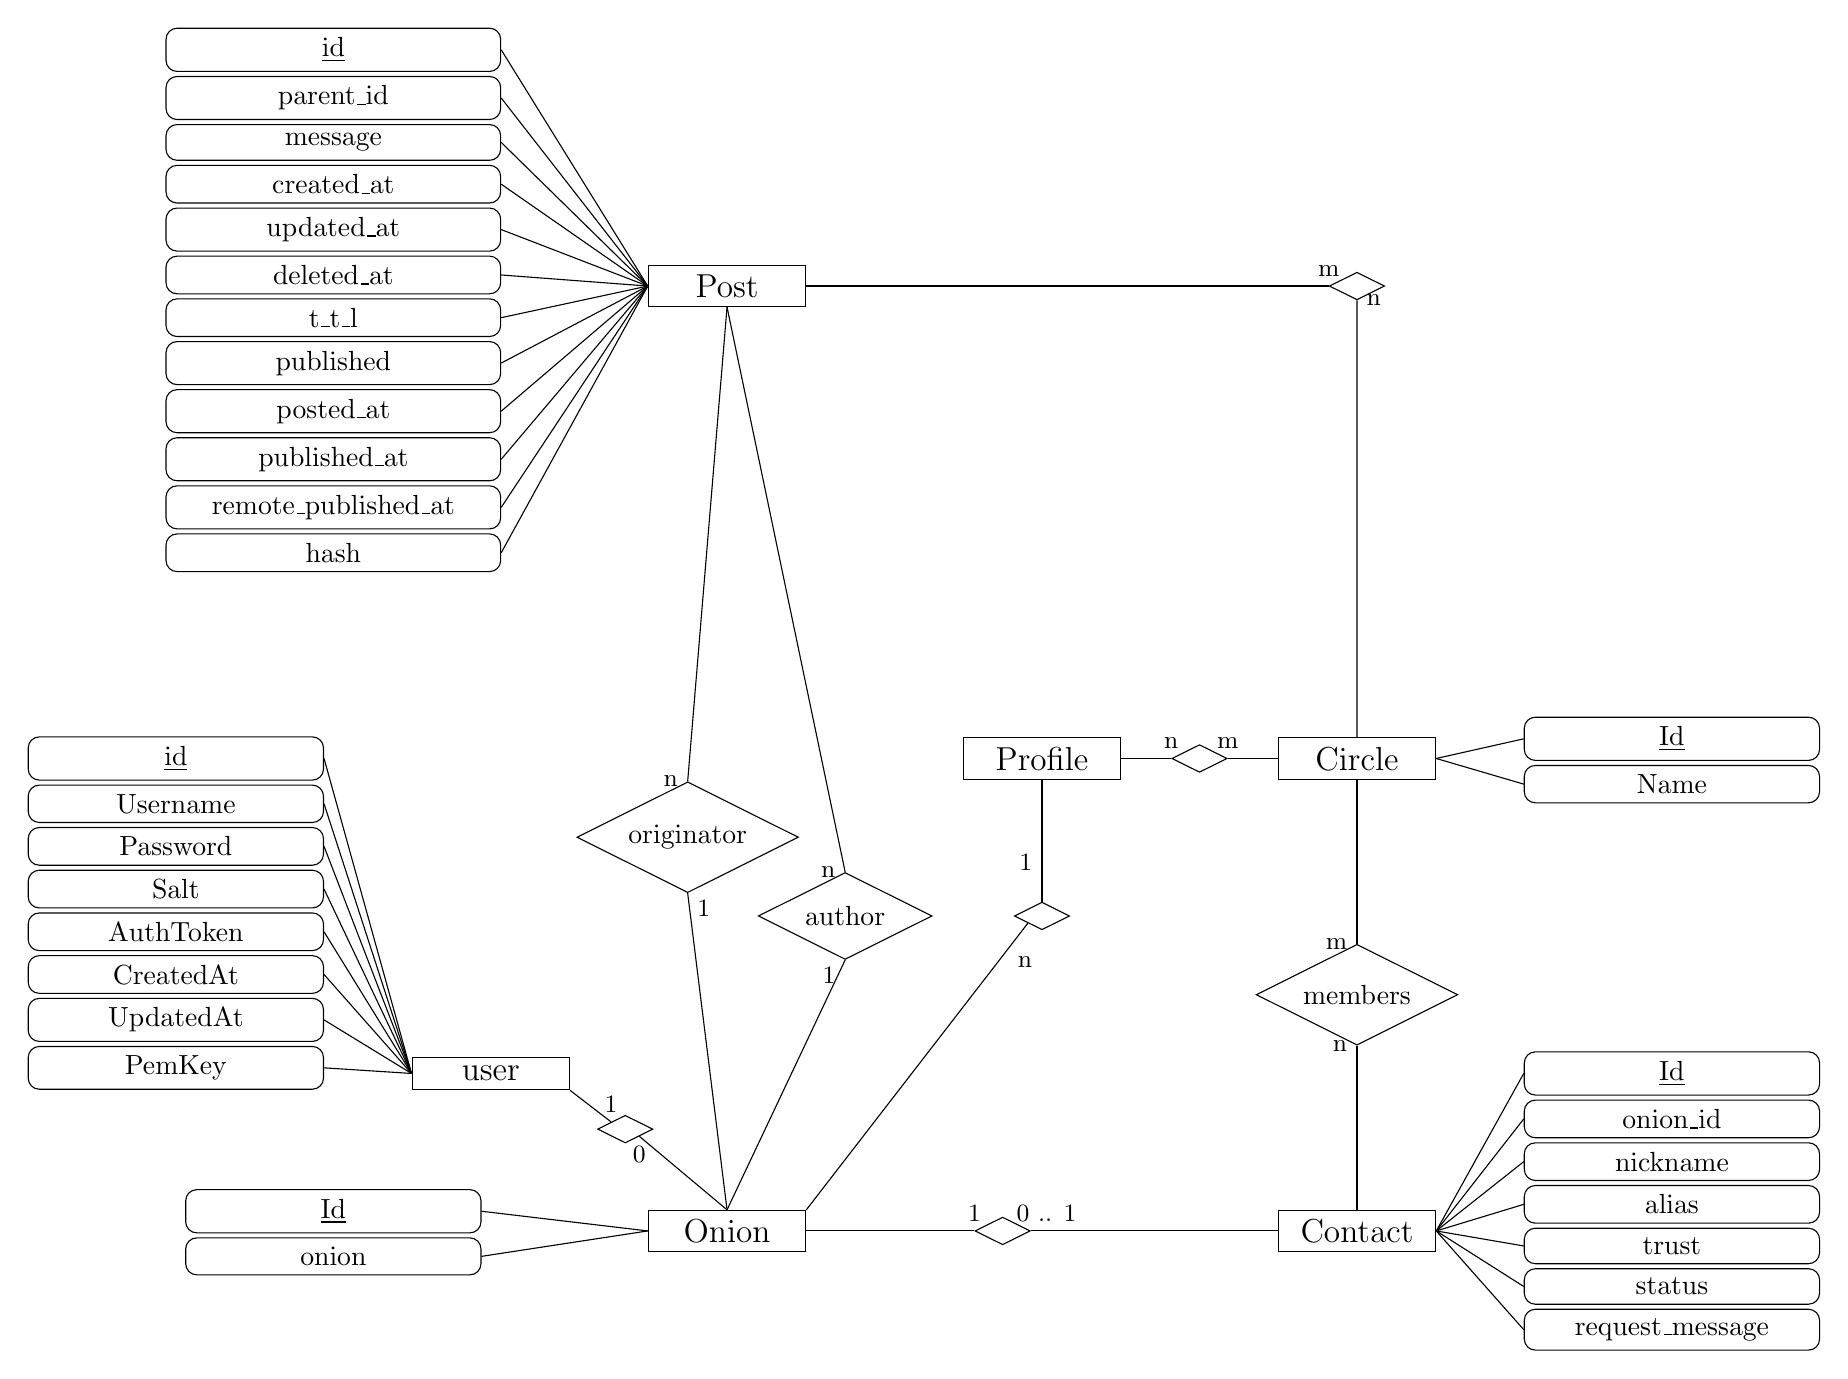
\begin{tikzpicture}
      \tikzstyle{field}=[font={\texttt\tiny}, rounded corners, draw, rectangle, minimum width=3.75cm]
      \tikzstyle{relation}=[draw, diamond, shape aspect=2]
      \tikzstyle{table}=[draw, font=\large, minimum width= 2cm]
      
      \node[table] (post) at (1cm, 2cm) {\large{Post}};

      \tikzset{postfield/.style={field, minimum width=4.25cm, append after command={(\tikzlastnode.east)edge(post.west)}}};
      
      \begin{scope}[node distance = .05cm, start chain=post going below, xshift=-4cm, yshift=5cm]
        \node[on chain=post, postfield] {\underline{id}};
        \node[on chain=post, postfield] {parent\_id};
        \node[on chain=post, postfield] {message};
        \node[on chain=post, postfield] {created\_at};
        \node[on chain=post, postfield] {updated\_at};
        \node[on chain=post, postfield] {deleted\_at};
        \node[on chain=post, postfield] {t\_t\_l};
        \node[on chain=post, postfield] {published};
        \node[on chain=post, postfield] {posted\_at};
        \node[on chain=post, postfield] {published\_at};
        \node[on chain=post, postfield] {remote\_published\_at};
        \node[on chain=post, postfield] {hash};
      \end{scope}

      \node[table] (user) at (-2cm, -8cm) {\large{user}};
      \tikzset{userfield/.style={on chain=user, field, append after command={(\tikzlastnode.east)edge(user.west)}}};
      \begin{scope}[node distance = .05cm, start chain=user going below, xshift=-6cm, yshift=-4cm]
        \node[userfield] {\underline{id}};
        \node[userfield] {Username};
        \node[userfield] {Password};
        \node[userfield] {Salt};
        \node[userfield] {AuthToken};
        \node[userfield] {CreatedAt};
        \node[userfield] {UpdatedAt};
        \node[userfield] {PemKey};
      \end{scope}

      
      \node[table] (circle) at (9cm, -4cm) {Circle};
      
      % Post <-> Circle relation
      \node[relation, right of=post, node distance=8cm] (postcircles) {};
      \draw (post.east) -- (postcircles.west) node[above] {\small{m}};
      \draw (circle.north) -- (postcircles.south) node[right] {\small{n}};

      \tikzset{circlefield/.style={field, on chain=circle, append after command={(\tikzlastnode.west)edge(circle.east)}}};
      \begin{scope}[node distance = .05cm, start chain=circle going below, xshift=13cm, yshift = -3.75cm]
        \node[circlefield] {\underline{Id}};
        \node[circlefield] {Name};
      \end{scope}


      \node[table] (contact) at( 9cm, -10cm) {Contact};
      \tikzset{contactfield/.style={field, on chain=contact, append after command={(\tikzlastnode.west)edge(contact.east)}}};
      \begin{scope}[node distance = .05cm, start chain=contact going below, xshift=13cm, yshift = -8cm]
        \node[contactfield] {\underline{Id}};
        \node[contactfield] {onion\_id};
        \node[contactfield] {nickname};
        \node[contactfield] {alias};
        \node[contactfield] {trust};
        \node[contactfield] {status};
        \node[contactfield] {request\_message};
      \end{scope}

      \node[relation, above of=contact, node distance=3cm] (members) {members};
      \draw (contact.north) -- (members.south) node[left] {\small{n}};
      \draw (circle.south) -- (members.north) node[left] {\small{m}};

      \node[table] at (1cm, -10cm) (onion) {Onion};
      \tikzset{onionfield/.style={field, on chain=onion, append after command={(\tikzlastnode.east)edge(onion.west)}}};
      \begin{scope}[node distance = .05cm, start chain=onion going below, yshift = -9.75cm, xshift=-4cm]
        \node[onionfield] {\underline{Id}};
        \node[onionfield] {onion};
      \end{scope}


      \node[relation, below right of=user, node distance = 1cm, xshift = 1cm] (useronion) {};
      \draw (user.south east) -- (useronion.north west) node[right, above] {\small{1}};
      \draw (onion.north) -- (useronion.south east) node[left, below] {\small{0}};
      
      \node[relation] (contonion) at (4.5cm, -10cm) {};
      \draw (onion.east) -- (contonion.west) node[above] {\small{1}};
      \draw (contact.west) -- (contonion.east) node[above, xshift=.2cm] {\small{0 .. 1}};

      \node[relation] (author) at (2.5cm, -6cm) {author};
      \node[relation] (orig) at (0.5cm, -5cm) {originator};

      \draw (onion.north) -- (author.south) node[left, yshift=-.2cm] {\small{1}};
      \draw (onion.north) -- (orig.south) node[right, yshift=-.2cm] {\small{1}};
      \draw (post.south) -- (author.north) node[left] {\small{n}};
      \draw (post.south) -- (orig.north) node[left] {\small{n}};

      \node[table, left of=circle, node distance = 4cm] (profile) {Profile};
      \node[relation, right of = profile, node distance = 2cm] (profcirc) {};
      \draw (profile.east) -- (profcirc.west) node[above] {\small{n}};
      \draw (circle.west) -- (profcirc.east) node[above] {\small{m}};

      \node[relation, below of=profile, node distance=2cm] (profonion) {};
      \draw (profile.south) -- (profonion.north) node[left,yshift=.5cm] {\small{1}};
      \draw (onion.north east) -- (profonion.south west) node[right, yshift=-.5cm, xshift=-.25cm] {\small{n}};
    \end{tikzpicture}
    \caption{Entity Relationship Model}
  \end{figure}
\end{landscape}

\input{parts/frontend}
\input{parts/apidocs}

\section{Security Considerations}

\subsection{Reliance on Tor}
\label{tor_security}
The Zwiebelnetz heavily relies on Tor's security. The systems build a friend-to-friend network among contacts, making it easy to extract the social graph from connection data. If Tor traffic can be de-anonymized, the encrypted traffic could potentially reveal private information such as:
\begin{itemize}
  \item Who is a contact of whom, since communication only happens between contacts.
  \item When does someone post (or update the profile): Very short message sent to contacts is likely a ``Trigger'' packet.
  \item How long is a Post, or how many Profile updates were written: TCP Connections are closed right after a Pull request is served. The more data there is to send, the more encrypted traffic will pass the network.
  \item Who do you post to or publish profiles entries to: The Trigger messages are only sent to valid recipients if a Post is written or a profile entry is updated.
\end{itemize}
Many more such information could potentially be extracted if Tor's anonymization was broken.

We also rely on Tor's promise to protect data's authenticity, integrity and privacy for data sent to hidden services and the one-way authentication. Tor uses RSA keys with a length of 1024 bit to secure the initial diffie-hellman key exchange upon new connections. RSA-1024 is no longer conisidered secure nowadays.

Also, we rely on the uniqueness of onion addresses. We do not store other system's public keys - we only store the onion address. During authentication (see \autoref{authentication}), the requested system sends it's public key. We only check that the onion of the public key indeed matches the onion we stored. If it was possible to generate a public key with yields the same onion address, attacker could have us connect and authenticate to his system, allowing to send us posts not written by the contact we think they were. He would also be able to authenticate to us, since the syncer server, as well, only checks if the key passed with the \texttt{Auth} package matches the onion address of a contact. This would allow the attacker to obtain any information the impersonated contact could read. Onion addresses in Tor are the \textit{first 80 bit} only of the 160 bit \texttt{SHA1}-hash. In general, the security parameters seem to be set rather low with Tor. There are proposals in the Tor project to switch to longer onion addresses and use elliptic curve public key cryptography. Most of our code is compatible with such changes, so that a transition to different onion length or different public key cryptography schemes would affect few components.

Two ideas to improve on security problems caused by Tor are:
\begin{itemize}
\item Do not reply on Tor's transport security, tunnel through TLS or similiar. This would require to use some concatenation of onion address and some TLS certificate fingerprint as contact information.
\item Store public keys of contacts. If an attacker generates a key pair with the same onion address in the future, it will not match the stored public key and be rejected.
\end{itemize}

\subsection{Markdown}

We support markdown for Posts and Comments. This enables the creation of well formated postings instead of just text messages. The markdown library consists is a Javascript based parser which converts the posts into html in the browser of the viewing user. Security bugs in the markdown library would allow only Contacts to attack the viewing client. While not as critical as attacks which \textit{any} user, not only contacts, could run, an the (unaudited) markdown parser should be disabled if of concern.

One issue we encountered is the inline rendering of external images. It allows malicious contacts to link to images on own web servers with unique urls and later analyze the server logs. This could be used to identify IP addresses of users which keep the attackers as contact of follow him.

This affects the comment functionality. An attacker use this to read the IP addresses of the contacts and followers of a \textit{contact} of his.

An easy way to protect against this attack is to enable Tor in the browser which accesses the Zwiebelnetz, the server logs will only show anonymous connections via the Tor network. The number of connections, however, will not be hidden this way.

\subsection{Unaudited Code Base}

Our code-base consists of more than five thousand lines of \texttt{golang} and several web languages. Only some parts of the code were read by another team member after being written. It is therefore likely, that the code-base contains unknown security issues.

While the syncer and restful API mostly use the standard library of \texttt{golang}, the frontend uses a large web framework and several web components. While all of those are commonly used on the Internet, it is not clear to us how much their code can be trusted.

\subsection{Frontend Connectivity}

The frontend connects to the JSON-API using plain HTTP, not HTTPS. It is therefore suggested to manually set up a second Tor hidden service which is used to connect firstly in a secure manner (see \autoref{tor_security}, though) and secondly from a remote location, outside the local area network, which, in our case, usually is a home environment.

Authentication is done via salted hashes using \texttt{SHA-256} as a hash function. In the plain HTTP case, this means that passwords are transmitted as plaintext. While plaintext passwords are only transmitted in the LAN environment, this is still undesirable, the user could connect to his system using shared wireless connection. Again, use a second Tor hidden service for frontend connectivity.

The browser stores an access token in a cookie after authentication. This cookie allows the frontend to authenticate to the JSON-API without the user having to enter his password every few seconds. If the user does not protect physical access to his device, an attacker could use the Zwiebelnetz without loggin in, though, as long as a browser with a Zwiebelnetz session is still open.

\section{Used Software, Frameworks and Libraries}

\subsection{BackEnd}
The backend was developed in Go [\url{https://www.golang.org/}], an open source programming language. The following libraries were used.
  \begin{itemize}
    \item Go-Json-Rest [\url{https://github.com/ant0ine/go-json-rest/}],\\a quick and easy way to setup a RESTful JSON API
    \item go-sqlite3 [\url{https://github.com/mattn/go-sqlite3}],\\sqlite3 driver conforming to the built-in database/sql interface.
    \item GORM [\url{https://github.com/jinzhu/gorm}],\\object-relational mapping library for Go.
  \end{itemize}

\subsection{FrontEnd}
\label{software_frontend}
The frontend is web-based and can be used with any conventional browser (Firefox, Chrome, Opera etc.). Techniques like HTML and JavaScript/CoffeeScript and the following libraries were used.
  \begin{itemize}
    \item jQuery [\url{http://jquery.com/}],\\a fast, small, and feature-rich JavaScript library.
    \item Bootstrap [\url{http://getbootstrap.com/}],\\popular HTML, CSS, and JS framework.
    \item Ember.js [\url{http://emberjs.com/}],\\a framework for creating ambitious web application.
    \item Emblem.js [\url{ http://emblemjs.com/}],\\a new templating language that compiles to Handlebars.js. (Handlebars provides the power necessary to let you build semantic templates effectively with no frustration.)
    \item Moment.js [\url{http://momentjs.com/}],\\Parse, validate, manipulate, and display dates in JavaScript.
    \item marked [\url{https://github.com/chjj/marked}],\\a full-featured markdown parser and compiler.
    \item Select2 [\url{http://ivaynberg.github.io/select2/}],\\is a jQuery based replacement for select boxes.
  \end{itemize}

\bibliography{tech-report}
\bibliographystyle{plain}

\end{document}
